%-----------------------------------------------------------------------------
%
%               Template for sigplanconf LaTeX Class
%
% Name:         sigplanconf-template.tex
%
% Purpose:      A template for sigplanconf.cls, which is a LaTeX 2e class
%               file for SIGPLAN conference proceedings.
%
% Guide:        Refer to "Author's Guide to the ACM SIGPLAN Class,"
%               sigplanconf-guide.pdf
%
% Author:       Paul C. Anagnostopoulos
%               Windfall Software
%               978 371-2316
%               paul@windfall.com
%
% Created:      15 February 2005
%
%-----------------------------------------------------------------------------

\documentclass{sigplanconf}

% The following \documentclass options may be useful:

% preprint      Remove this option only once the paper is in final form.
%10pt          To set in 10-point type instead of 9-point.
% 11pt          To set in 11-point type instead of 9-point.
% authoryear    To obtain author/year citation style instead of numeric.

\usepackage{amsmath}
\usepackage{epsfig}
\usepackage{alltt}
\usepackage{times}
\usepackage{array}
\usepackage{algorithm}
\usepackage{algorithmic}
\usepackage{graphicx}


\newlength\myindent
\setlength\myindent{1em}
\newcommand\bindent{%
  \begingroup
  \setlength{\itemindent}{\myindent}
  \addtolength{\algorithmicindent}{\myindent}
}
\newcommand\eindent{\endgroup}

\newlength\mysecindent
\setlength\mysecindent{2em}
\newcommand\quadindent{%
  \begingroup
  \setlength{\itemindent}{\mysecindent}
  \addtolength{\algorithmicindent}{\mysecindent}
}
\newcommand\quadeindent{\endgroup}


\begin{document}

\special{papersize=8.5in,11in}
\setlength{\pdfpageheight}{\paperheight}
\setlength{\pdfpagewidth}{\paperwidth}

\conferenceinfo{CONF 'yy}{Month d--d, 20yy, City, ST, Country} 
\copyrightyear{20yy} 
\copyrightdata{978-1-nnnn-nnnn-n/yy/mm} 
\doi{nnnnnnn.nnnnnnn}

% Uncomment one of the following two, if you are not going for the 
% traditional copyright transfer agreement.

%\exclusivelicense                % ACM gets exclusive license to publish, 
                                  % you retain copyright

%\permissiontopublish             % ACM gets nonexclusive license to publish
                                  % (paid open-access papers, 
                                  % short abstracts)

\titlebanner{banner above paper title}        % These are ignored unless
\preprintfooter{short description of paper}   % 'preprint' option specified.

\title{Parallelized Regressions}
\subtitle{Subtitle Text, if any}

\authorinfo{Abhishek Agarwal}
           {University of Texas at Austin}
           {abhishek.agarwal@utexas.edu}
\authorinfo{Ankit Goyal}
           {University of Texas at Austin}
           {ankit3goyal@gmail.com}
\authorinfo{Prateek Agarwal}
           {University of Texas at Austin}
           {prat0318@gmail.com}

\maketitle

\begin{abstract}
The main focus of this work is to solve the problem of Regression for Sparse Data-sets using the Galois framework.
To the best of our knowledge, this is the first attempt at implementing parallel Regression Algorithms using
Galois. Two different solvers; Gradient and Coordinate descent and their stochastic versions are implemented. The
algorithms are parallelized using OpenMP and Galois framework and their performance and accuracy are compared.
The Tao Analysis for the two solvers is presented and Speedup is compared for different Galois worklist scheduling. A
comparative analysis is presented for change in error loss with respect to the number of iterations and threads. 
\end{abstract}

\category{CR-number}{subcategory}{third-level}

\keywords
keyword1, keyword2

\section{Introduction}

\section{Related Work}
Several papers were written recently studying the iteration complexity of serial CDMs of various flavours and in various settings. 
We will only provide a brief summary here, for a more detailed account we refer the reader to [16]. Classical CDMs update the coordinates in a cyclic order; 
the first attempt at analyzing the complexity of such a method is due to [21]. Stochastic/randomized CDMs, that is, methods where
the coordinate to be updated is chosen randomly, were first analyzed for quadratic objectives [24,4], later independently generalized to
L1-regularized problems [23] and smooth block-structured problems [10], and finally unified and refined in [19, 16]. 
The problems considered in the above papers are either unconstrained or have (block) separable constraints. Recently, randomized CDMs
were developed for problems with linearly coupled constraints [7, 8]. A greedy CDM for L1-regularized problems was 
first analyzed in [15]; more work on this topic include [5, 2]. A CDM with inexact updates was first proposed and analyzed in [26]. Partially
separable problems were independently studied in [13], where an asynchronous parallel stochastic
gradient algorithm was developed to solve them.
When writing this paper, the authors were aware only of the parallel CDM proposed and analyzed in [1]. Several papers on the 
topic appeared around the time this paper was finalized or after [6, 28, 22, 22, 14]. Further papers on various aspects of the 
topic of parallel CDMs, building on the work in this paper, include [25, 17, 3, 18].

\section{Regression}
\noindent
Regression models and analyzes the correlation of several variables. Given a set of training examples 
\begin{math}(x_1,y_1),....,(x_n,y_n)\end{math} where \begin{math} x_i \in R^n \end{math}
and \begin{math} y_i \in (-1,1) \end{math},the goal is to learn a linear scoring function
\begin{math} f(x) = w^Tx + b \end{math} with model parameters \begin{math} w \in R^m \end{math}
and intercept \begin{math} b \in R. \end{math}\\

\noindent
A common choice to find the model parameters is by minimizing the regularized training error given by\\
\begin{equation} E(w,b) = \sum_{i=1}^{n} L(y_i,f(x_i)) + \alpha R(w) \end{equation} \\
where L is a loss function that measures models' (mis)fit and \begin{math}R\end{math} is a
regularization term (aka penalty) that penalizes model complexity; \begin{math}\alpha>0\end{math}
is a non-negative hyperparameter.

\section{Models for Regression}
\subsection{Least Squares}
The best fitting curve to a set of data points could be obtained using least square method. The method
assumes that the best-fit curve for a given data has the minimal sum of the deviations squared. It could
be represented as a minimization problem. For Least squares, the regularization function \begin{math}R(w)=0\end{math}
such that the error is given by \\
\begin{equation} E(w,b) =\frac{1}{2} \sum_{i=1}^{n} (y-Ax)^2\end{equation}
Least Squares has the problem of Overfitting leading to a model that fits the training data very well, but does not generalize well (predict accurately for new examples).

\subsection{Regularization for Regression}
Regularization refers to a process of introducing additional information in order to solve an ill-posed problem or to prevent overfitting. 
This information is usually of the form of a penalty for complexity, such as restrictions for smoothness or bounds on the vector space norm.
For Regression, various Regularization models are used as described next.

\subsubsection{Ridge Regression}
Ridge regression penalizes the size of the regression coefficients. Applying the ridge regression penalty
has the effect of shrinking the estimates (introducing bias but reducing the variance of the estimate). The Error
function is given by \\
\begin{equation} E(w,b) =\frac{1}{2} \sum_{i=1}^{n} (y-Ax)^2 + \sum_{i=1}^{n} w_i^2 \end{equation} \\
The Regularization function is
\begin{equation}R(w)=\frac{1}{2} \sum_{i=1}^{n} w_i^2\end{equation}.

\subsubsection{Lasso}
Ridge regression is capable of reducing the variability and improving the accuracy of linear regression
models, and that these gains are largest in the presence of multicollinearity. However ridge regression
doesn't do variable selection, and it fails to provide a parsimonious model with few parameters.
LASSO is a regression method that penalizes the absolute size of the regression coefficients. It has
desirable effect of setting coefficients to zero leading to sparse solutions.\\
\begin{equation} E(w,b) =\frac{1}{2} \sum_{i=1}^{n} (y-Ax)^2 + \sum_{i=1}^{n} w_i \end{equation} \\
The Regularization function is
\begin{equation}R(w)=\sum_{i=1}^{n} |w_i|\end{equation}.

\subsection{Elastic Net}
Elastic net is a linear model that allows for learning a sparse model where few of the weights are nonzero
like Lasso, while still maintaining the regularization properties of Ridge. The Error function is given by
\begin{equation}E(w,b) =\frac{1}{2} \sum_{i=1}^{n} (y-Ax)^2 + \sum_{i=1}^{n} w_i^2 + \sum_{i=1}^{n} w_i \end{equation} \\
The Regularization function is
\begin{equation}R(w) = \gamma \frac{1}{2} \sum_{i=1}^{n} w_i^2 + (1-\gamma)\sum_{i=1}^{n} |w_i|\end{equation}.

\section{Solvers for Regression}
\subsection{Exact Solvers}
Different libraries for matrix computation and linear algebra operations
Default BLAS and LAPACK, used by Octave
Intel Math Kernel Library (Intel MKL), used by Matlab
AMD Core Math Library (ACML)
Automatically Tuned Linear Algebra Software (ATLAS)
Closed form solution:- \begin {math} O(nd^2 + d^3) \end {math} time and \begin {math} O(d^2) \end {math} space for linear regression
Not scalable for large number of features (d).

\subsection{Gradient Descent}
To find a local minimum of a function using gradient descent, one takes steps proportional to the negative of 
the gradient (or of the approximate gradient) of the function at the current point. The gradient of the error 
function is taken w.r.t one sample at a time and the new weight value for all features is computed.
At the end of the iteration, the final weight values are updated with the mean of weight values calculated using all samples.

\begin{algorithm}
\caption{	Gradient Descent}
\begin{algorithmic} 

\STATE \bf{INPUT} \begin{math} X \in {R}^{N \times  d}, y \in R^N, learning\;  rate\;  \eta, intial\; w \end{math} 
\STATE \bf{OUTPUT} \textnormal{Solution} \begin{math}  w \end{math} 
	\STATE \textnormal{\begin{math} t = 0\end{math} }
	\STATE \bf{while} \textnormal{not converged} \bf{do}
    	\bindent
		 \STATE \bf{for} \textnormal{\indent training example \begin{math}1,2,3..k\end{math}}
		\quadindent
			 \STATE \textnormal{\indent Compute gradient for \begin{math}x_i: \bigtriangledown{E_w(x_i)}\end{math}}
			 \STATE \textnormal{\indent Update \begin{math}w: w^{(t+1)} \gets w^{(t)} - \bigtriangledown{E_w(x_i)}\end{math}}
			 \STATE \textnormal{\indent \begin{math}t \gets t + 1\end{math}}
		\quadeindent
	 \STATE \bf{end for}
	 \eindent
\STATE \bf{end while}

\end{algorithmic}
\end{algorithm}


\subsection{Stochastic Gradient Descent}
In stochastic (or "on-line") gradient descent, the true gradient of the function is approximated by a gradient at a
single training sample. The training samples are given one at a time. The algorithm examines the
current datapoint, and then updates the weight vector accordingly.
current datapoint, and then updates the weight vector accordingly. Thus, it is different from Gradient Descent where the weight
vector is updated with the mean of all samples.

\begin{algorithm}
\caption{Stochastic Gradient Descent}
\begin{algorithmic} 

\STATE \bf{INPUT} \begin{math} X \in {R}^{N \times  d}, y \in R^N, learning\;  rate\;  \eta, intial\; w \end{math} 
\STATE \bf{OUTPUT} \textnormal{Solution} \begin{math}  w \end{math} 

	\STATE \textnormal{\begin{math} t = 0\end{math} }

	\STATE \bf{while} \textnormal{not converged} \bf{do}
    	\bindent
	 \STATE \textnormal{\indent choose a random training example \begin{math}x_i\end{math}}

	 \STATE \textnormal{\indent Compute gradient for \begin{math}x_i: \bigtriangledown{E_w(x_i)}\end{math}}
	 \STATE \textnormal{\indent Update \begin{math}w: w^{(t+1)} \gets w^{(t)} - \bigtriangledown{E_w(x_i)}\end{math}}
	 \STATE \textnormal{\indent \begin{math}t \gets t + 1\end{math}}
	    \eindent
	\STATE \bf{end while}

\end{algorithmic}
\end{algorithm}

\subsection{Coordinate Descent}
As described in \cite{fried1}, Coordinate descent methods (CDM) are one of the most successful classes of algorithms in the big data optimization domain. 
Broadly speaking, CDMs are based on the strategy of updating a single coordinate (or a single block of coordinates) of the vector
of variables at each iteration. This often drastically reduces memory requirements as well as the
arithmetic complexity of a single iteration, making the methods easily implementable and scalable.
On the other hand, many more iterations are necessary for convergence than it is usual for classical gradient methods.
Coordinate descent is a non-derivative optimization algorithm. To find a local minimum of a function, one does line 
search along one coordinate direction at the current point in each iteration. One uses different coordinate directions 
cyclically throughout the procedure. On non-separable functions the algorithm may fail to find the optimum in a reasonable 
number of function evaluations. 
Coordinate descent is based on the idea that the minimization of a multi-variable function can be
achieved by minimizing it along one direction at a time. Its different from the gradient descent as instead of varying descent direction according
to gradient, one fixes descent direction at the outset.
\begin{algorithm}
\caption{Coordinate descent}
\begin{algorithmic} 
\STATE let $w = 0$
\STATE \bf{for} \begin{math} k = 1,2,.. \end{math}
    \bindent
	\STATE \bf{for} \textnormal{\begin{math}j\end{math} in \begin{math}\{1,...,2d\}\end{math}}
		\quadindent
	\STATE \textnormal{let \begin{math}g_j = (\bigtriangledown{E(w)})_j\end{math}}
	\STATE \textnormal{let \begin{math}\eta = max\{ -w_j, -g_j/\beta \}\end{math}}
	\STATE \textnormal{let \begin{math}w_j = w_j + \eta\end{math}}
	\quadeindent
	\STATE \bf{end for}
    \eindent
\STATE \bf{end for}
\end{algorithmic}
\end{algorithm}


\subsection{Stochastic Coordinate Descent}
If the number of features and data sets is large, going over all dimensions in each iteration is an
expensive approach. In Stochastic Coordinate Descent, only one feature is updated at each iteration. The 
features to be updated can be choosen randomly or in a cyclic manner. The algorithm used for SCD is 
described below.

\begin{algorithm}
\caption{Stochastic coordinate descent}
\begin{algorithmic} 
\STATE let $w = 0$
\STATE \bf{for} \begin{math} k = 1,2,.. \end{math}
    \bindent
	\STATE \textnormal{sample \begin{math}j\end{math} uniformly at random from \begin{math}\{1,...,2d\}\end{math}}
	\STATE \textnormal{let \begin{math}g_j = (\bigtriangledown{E(w)})_j\end{math}}
	\STATE \textnormal{let \begin{math}\eta = max\{ -w_j, -g_j/\beta \}\end{math}}
	\STATE \textnormal{let \begin{math}w_j = w_j + \eta\end{math}}
    \eindent
\STATE \bf{end for}
\end{algorithmic}
\end{algorithm}

\section{Parallel Implementation}
\subsection{Parallel Stochastic Gradient Descent}
\subsection{Parallel Stochastic Coordinate Descent}

\section{TAO Analysis}
\subsection{Parallel Stochastic Gradient Descent}
\subsection{Parallel Stochastic Coordinate Descent}

\section{Implementation Framework}
\subsection{OpenMP}
\subsection{Galois System}
\subsection{Scikit Runs}
\subsection{Stampede}

\section{Datasets}
\subsection{Mnist}
\begin{figure}[ht!]
\centering
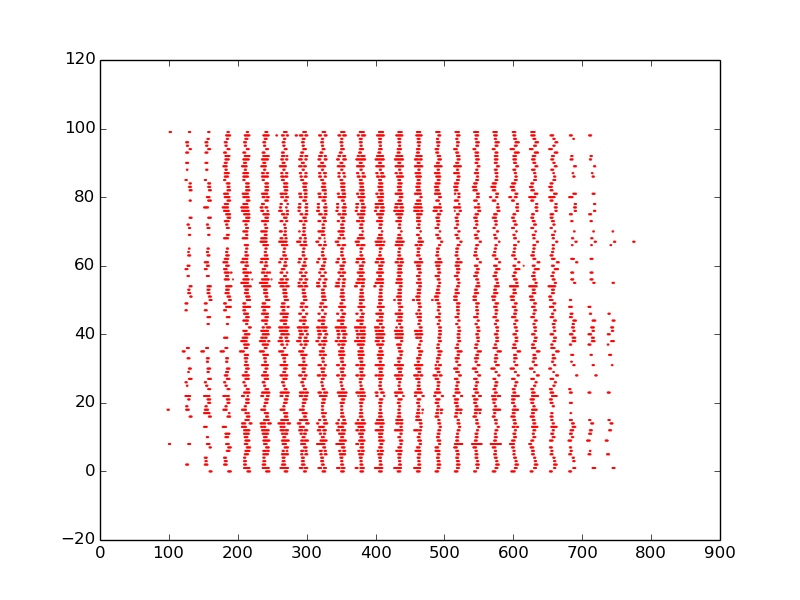
\includegraphics[width=80mm]{mnist_scatter.png}
\caption{Sparse representation of a small set of samples from MNIST. X axis represents the feature present, Y axis represents a sample for which features are present. }
\label{overflow}
\end{figure}

MNIST is a sparse dataset(9\% of the total data-set are non-zero values). This data was primarily built for classification analysis. The database was constructed from NIST's Special Database 3 and Special Database 1 which contain binary images of handwritten digits. The variable set consists of all pixels used to form the digit image. We transformed the data for regression by selecting only two digit samples, namely 1 and 9 and then using it as a binary regression. Samples for 1 were given a Y value of 1 and samples for 9 were given a Y value of -1. Total feature size of the samples is 800 and the total number of samples used were around 0.5 million (513280 samples). Value of any X feature lies in the range(0,255).

\subsection{Madelon}
Madelon is a dense dataset, with number of features kept comparable to the number of samples. It was generated by the program hypercube\_data.m. Some co-variance is added by multiplying the generated data by a random matrix A, with uniformly distributed random numbers between -1 and 1. The samples have been assigned Y values such that half of the samples are assigned 1 as Y value and the other half as -1 as Y value.Total feature size of the samples is 500 and the total number of samples used were 5000. Values of any X feature lies in the range(0,999).

\section{TAO Analysis}

\begin{table}[htbp]
\caption{Run time for GD on MNIST dataset}
\begin{tabular}{|l|r|r|r|r|r|}
\hline
 & 1 & 2 & 4 & 8 & 16 \\ \hline
Galois Chunked FIFO & 45.96 & 30.36 & 20.53 & 16.08 & 12.53 \\ \hline
Galois dChunked FIFO & 43.46 & 26.55 & 15.26 & 8.33 & 6.33 \\ \hline
Galois FIFO & 32.5433 & 24.79 & 19.76 & 17.54 & 16.38 \\ \hline
OPENMP & 15.72 & 7.184 & 3.70 & 2.30 & 1.31 \\ \hline
OPENMP Chunked. & 15.55 & 6.83 & 3.49 & 2.12 & 1.13 \\ \hline
\end{tabular}
\end{table}

\subsection{Parallel Stochastic Gradient Descent}
\begin{table}[htbp]
\caption{Run time for SGD on MNIST dataset}
\begin{tabular}{|l|r|r|r|r|r|}
\hline
 & 1 & 2 & 4 & 8 & 16 \\ \hline
Galois CHUNKED FIFO & 38.43 & 21.24 & 12.32 & 6.39 & 4.11 \\ \hline
Galois FIFO & 21.24 & 20.09 & 17.81 & 16.38 & 15.88 \\ \hline
OPENMP & 6.97 & 3.38 & 1.83 & 1.04 & 0.63 \\ \hline
\end{tabular}
\label{Label of the table}
\end{table}



\subsection{Parallel Stochastic Coordinate Descent}

\begin{table}[htbp]
\caption{Runtime for SCD on Madelon dataset}
\begin{tabular}{|l|r|r|r|r|r|}
\hline
 & 1 & 2 & 4 & 8 & 16 \\ \hline
Galois - LC\_CSR & 349.69 & 204.94 & 123.65 & 84.76 & 261.08 \\ \hline
Galois - STL::Vector  & 35.80 & 32.06 & 32.06 & 31.95 & 36.24 \\ \hline
OPENMP & 22.14 & 37.08 & 17.4413 & 9.02 & 5.66 \\ \hline
\end{tabular}
\label{Label of the table}
\end{table}


\section{Parallel Implementation}
\subsection{Parallel Gradient Descent}
\subsection{Parallel Stochastic Gradient Descent}
\subsection{Parallel Stochastic Coordinate Descent}
\begin{equation} \mu = \frac{y^T \bar{X_i} - \widehat{w_i}^T H e_i }{H_{ii} + 2\lambda} \end{equation}

\section{Results}
\subsection{Parallel Gradient Descent}
\subsubsection{Different Galois Schedules vs OpenMP}
\subsubsection{Different Regression Models vs Accuracy}
\subsubsection{No of Iterations vs Accuracy}
\subsection{Parallel Stochastic Gradient Descent}
\subsubsection{Different Galois Schedules vs OpenMP}
\subsubsection{Accuracy Comparsion for SGD vs GD}
\subsubsection{Error Rate Variation with Danmping Factor \(\eta\) }
\subsection{Parallel Stochastic Coordinate Descent}
\subsubsection{Different Galois Schedules vs OpenMP}

\section{Conclusion}

% We recommend abbrvnat bibliography style.
\bibliographystyle{abbrvnat}
% The bibliography should be embedded for final submission.

\begin{thebibliography}{}
\softraggedright

\bibitem[Zhang et~al.(2004) Zhang, T.]{zhang1}
Zhang T., Solving Large Scale Linear Prediction Problems Using Stochastic Gradient Descent Algorithms.
\bibitem[Niu et~al.(2011)Niu, F.]{niu1}
Niu F. and Recht B., Hogwild!: A Lock-Free Approach to Parallelizing Stochastic Gradient Descent.
\bibitem[Richtarik et~al.(2012) Richtarik, P.]{rich1}
Richtarik P., and Takac M., Parallel Coordinate Descent methods for Big Data Optimization.
\bibitem[Friedman et~al.(2007) Friedman, J.]{fried1}
J. Friedman, T. Hastie, H. Hoeing, and R. Tibshirani, Pathwise coordinate optimization.
\bibitem[Fu et~al.(1998) Fu, W.]{fu1}
W. Fu, Penalized regressions: the bridge versus the lasso.
\bibitem[Wu et~al.(2008) Wu, T.]{wu1}
T. Wu and K. Lange, Coordinate descent algorithms for lasso penalized regression.
\bibitem[Galois paper] {galois1}

\end{thebibliography}

\appendix

\section{Appendix Title}

This is the text of the appendix, if you need one.

\acks

Acknowledgments, if needed.

\end{document}

%                       Revision History
%                       -------- -------
%  Date         Person  Ver.    Change
%  ----         ------  ----    ------

%  2013.06.29   TU      0.1--4  comments on permission/copyright notices

